% Created 2016-12-09 Fr 23:09
\documentclass[a4paper]{scrartcl}
\usepackage[utf8]{inputenc}
\usepackage[T1]{fontenc}
\usepackage{fixltx2e}
\usepackage{graphicx}
\usepackage{longtable}
\usepackage{float}
\usepackage{wrapfig}
\usepackage{rotating}
\usepackage[normalem]{ulem}
\usepackage{amsmath}
\usepackage{textcomp}
\usepackage{marvosym}
\usepackage{wasysym}
\usepackage{amssymb}
\usepackage{hyperref}
\tolerance=1000
\usepackage{siunitx}%
\usepackage{fontspec}%
\sisetup{load-configurations = abbrevations}%
\newcommand{\estimates}{\overset{\scriptscriptstyle\wedge}{=}}%
\usepackage{mathtools}%
\DeclarePairedDelimiter\abs{\lvert}{\rvert}%
\DeclarePairedDelimiter\norm{\lVert}{\rVert}%
\DeclareMathOperator{\Exists}{\exists}%
\DeclareMathOperator{\Forall}{\forall}%
\def\colvec#1{\left(\vcenter{\halign{\hfil$##$\hfil\cr \colvecA#1;;}}\right)}
\def\colvecA#1;{\if;#1;\else #1\cr \expandafter \colvecA \fi}
\usepackage{minted}
\usepackage{makecell}
\usemintedstyle{perldoc}
\usepackage{tikz}
\usetikzlibrary{arrows,automata}
\usepackage{tikz-qtree}
\usepackage{enumitem}
\setlistdepth{20}
\renewlist{itemize}{itemize}{20}
\setlist[itemize]{label=$\cdot$}
\usepackage{amsthm}
\theoremstyle{definition}
\newtheorem{defn}{Definition}
\theoremstyle{plain}
\newtheorem{thm}{Satz}
\theoremstyle{remark}
\newtheorem{remark}{Bemerkung}
\theoremstyle{remark}
\newtheorem{ex}{Beispiel}
\usepackage{etoolbox}
\patchcmd{\thmhead}{(#3)}{#3}{}{}
\usepackage{xparse}% http://ctan.org/pkg/xparse
\NewDocumentCommand{\overarrow}{O{=} O{\uparrow} m}{%
\overset{\makebox[0pt]{\begin{tabular}{@{}c@{}}#3\\[0pt]\ensuremath{#2}\end{tabular}}}{#1}
}
\NewDocumentCommand{\underarrow}{O{=} O{\downarrow} m}{%
\underset{\makebox[0pt]{\begin{tabular}{@{}c@{}}\ensuremath{#2}\\[0pt]#3\end{tabular}}}{#1}
}
\renewcommand*{\proofname}{Beweis}
\author{Robin Heinemann}
\date{\today}
\title{Einführung in die Anwendungsorientierte Informatik (Köthe)}
\hypersetup{
  pdfkeywords={},
  pdfsubject={},
  pdfcreator={Emacs 25.1.1 (Org mode 8.2.10)}}
\begin{document}

\maketitle
\tableofcontents


\section{Was ist Informatik?}
\label{sec-1}
"Kunst" Aufgaben mit Computerprogrammen zu lösen.
\subsection{Teilgebiete}
\label{sec-1-1}
\subsubsection{theoretische Informatik (\textbf{ITH})}
\label{sec-1-1-1}
\begin{itemize}
\item Berechenbarkeit: Welche Probleme kann man mit Informatik lösen und welche prinzipiell nicht?
\item Komplexität: Welche Probleme kann man effizient lösen?
\item Korrektheit: Wie beweist man, dass das Ergebnis richtig ist? \\
      Echtzeit: Dass das richtige Ergebnis rechtzeitig vorliegt.
\item verteilte Systeme: Wie sichert man, dass verteilte Systeme korrekt kommunizieren?
\end{itemize}
\subsubsection{technische Informatik (\textbf{ITE})}
\label{sec-1-1-2}
\begin{itemize}
\item Auf welcher Hardware kann man Programme ausführen, wie baut man dies Hardware?
\item CPU, GPU, RAM, HD, Display, Printer, Networks
\end{itemize}
\subsubsection{praktische Informatik}
\label{sec-1-1-3}
\begin{itemize}
\item Wie entwickelt man Software?
\item Programmiersprachen und Compiler: Wie kommuniziert der Programmierer mit der Hardware?\hfill \textbf{IPI}, \textbf{IPK}
\item Algorithmen und Datenstrukturen: Wie baut man komplexe Programme aus einfachen Grundbausteinen?\hfill \textbf{IAL}
\item Softwaretechnik: Wie organisiert man sehr große Projekte?\hfill \textbf{ISW}
\item Kernanwendung der Informatik: Betriebssysteme, Netzwerke, Parallelisierung\hfill \textbf{IBN}
\begin{itemize}
\item Datenbanksysteme\hfill \textbf{IDB1}
\item Graphik, Graphische Benutzerschnittstellen\hfill \textbf{ICG1}
\item Bild- und Datenanalyse
\item maschinelles Lernen
\item künstliche Intelligenz
\end{itemize}
\end{itemize}
\subsubsection{angewandte Informatik}
\label{sec-1-1-4}
\begin{itemize}
\item Wie löst man Probleme aus einem anderem Gebiet mit Programmen?
\item Informationstechnik
\begin{itemize}
\item Buchhandlung, e-Kommerz, Logistik
\end{itemize}
\item Web Programmierung
\item scientific computing für Physik, Biologie
\item Medizininformatik
\begin{itemize}
\item bildgebende Verfahren
\item digitale Patientenakte
\end{itemize}
\item Computer Linguistik
\begin{itemize}
\item Sprachverstehen, automatische Übersetzung
\end{itemize}
\item Unterhaltung: Spiele, special effects im Film
\end{itemize}
\section{Wie unterscheidet sich Informatik von anderen Disziplinen?}
\label{sec-2}
\subsection{Mathematik}
\label{sec-2-1}
Am Beispiel der Definition $a \leq b: \exists c \geq 0: a + c = b$ \\
   Informatik: \\
   Lösungsverfahren: $a - b \leq 0$, das kann man leicht ausrechnen, wenn man subtrahieren und mit $0$ vergleichen kann. \\
   Quadratwurzel: $y = \sqrt{x} \iff y \geq 0 \wedge y^2 = x (\implies x > 0)$ \\
   Informatik: Algorithmus aus der Antike: $y = \frac{x}{y}$
iteratives Verfahren: \\
   Initial Guess $y^{(0)} = 1$
schrittweise Verbesserung $y^{(t+1)} = \frac{y^{(t)} + \frac{x}{y^{(t)}}}{2}$
\section{Informatik}
\label{sec-3}
Lösungswege, genauer Algorithmen
\subsection{Algorithmus}
\label{sec-3-1}
\textbf{schematische} Vorgehensweise mit der jedes Problem einer bestimmten \textbf{Klasse} mit \textbf{endliche} vielen \textbf{elementaren} Schritten / Operationen gelöst werden kann
\begin{itemize}
\item schematisch: man kann den Algorithmus ausführen, ohne ihn zu verstehen ($\implies$ Computer)
\item alle Probleme einer Klasse: zum Beispiel: die Wurzel aus jeder beliebigen nicht-negativen Zahl, und nicht nur $\sqrt{11}$
\item endliche viele Schritte: man kommt nach endlicher Zeit zur Lösung
\item elementare Schritte / Operationen: führen die Lösung auf Operationen oder Teilprobleme zurück, die wir schon gelöst haben
\end{itemize}
\subsection{Daten}
\label{sec-3-2}
Daten sind Symbole,
\begin{itemize}
\item die Entitäten und Eigenschaften der realen Welt im Computer repräsentieren.
\item die interne Zwischenergebnisse eines Algorithmus aufbewahren
\end{itemize}
$\implies$ Algorithmen transformieren nach bestimmten Regeln die Eingangsdaten (gegebene Symbole) in Ausgangsdaten (Symbole für das Ergebnis).
Die Bedeutung / Interpretation der Symbole ist dem Algorithmus egal $\estimates$ "schematisch"
\subsubsection{Beispiele für Symbole}
\label{sec-3-2-1}
\begin{itemize}
\item Zahlen
\item Buchstaben
\item Icons
\item Verkehrszeichen
\end{itemize}
aber: heutige Computer verstehen nur Binärzahlen $\implies$ alles andere muss man übersetzen
Eingansdaten: "Ereignisse":
\begin{itemize}
\item Symbol von Festplatte lesen oder per Netzwerk empfangen
\item Benutzerinteraktion (Taste, Maus, \ldots{})
\item Sensor übermittelt Messergebnis, Stoppuhr läuft ab
\end{itemize}
Ausgangsdaten: "Aktionen":
\begin{itemize}
\item Symbole auf Festplatte schreiben, per Netzwerk senden
\item Benutzeranzeige (Display, Drucker, Ton)
\item Stoppuhr starten
\item Roboteraktion ausführen (zum Beispiel Bremsassistent)
\end{itemize}
Interne Daten:
\begin{itemize}
\item Symbole im Hauptspeicher oder auf Festplatte
\item Stoppuhr starten / Timeout
\end{itemize}
\subsection{Einfachster Computer}
\label{sec-3-3}
endliche Automaten (endliche Zustandsautomaten)
\begin{itemize}
\item befinden sich zu jedem Zeitpunkt in einem bestimmten Zustand aus einer vordefinierten endlichen Zustandsmenge
\item äußere Ereignisse können Zustandsänderungen bewirken und Aktionen auslösen
\end{itemize}
\subsubsection{{\bfseries\sffamily TODO} Graphische Darstellung}
\label{sec-3-3-1}
graphische Darstellung: Zustände = Kreise, Zustandsübergänge: Pfeile
\subsubsection{{\bfseries\sffamily TODO} Darstellung durch Übergangstabellen}
\label{sec-3-3-2}
Zeilen: Zustände, Spalten: Ereignisse, Felder: Aktion und Folgezustände
\begin{center}
\begin{tabular}{llll}
Zustände $\backslash$ Ereignisse & Knopf drücken & Timeout & Timeout(Variante)\\
\hline
aus & $\implies$ \{halb\} \\ \{4 LEDs an\} & \% & ($\implies$ \{aus\},\{nichts\})\\
halb & ($\implies$ \{voll\},\{8 LEDs an\}) & \% & ($\implies$ \{aus\},\{nichts\})\\
voll & ($\implies$ \{blinken an\},\{Timer starten\}) & \% & ($\implies$ \{aus\},\{nichts\})\\
blinken an & ($\implies$ \{aus\},\{Alle LEDs aus, Timer stoppen\}) & ($\implies$ \{blinken aus\},\{alle LEDs aus, Timer starten\}) & ($\implies$ \{blinken aus\},\{8 LEDs aus\})\\
blinken aus & ($\implies$ \{aus\},\{Alle LEDs aus, Timer stoppen\}) & ($\implies$ \{blinken an\},\{alle LEDs an, Timer starten\}) & ($\implies$ \{blinken an\},\{8 LEDs an\})\\
\end{tabular}
\end{center}

Variante: Timer läuft immer (Signal alle 0.3s) $\implies$ Timout ignorieren im Zustand "aus", "halb", "voll"
\subsubsection{Beispiel 2:}
\label{sec-3-3-3}
\begin{align}
&1~0~1~1~0~1~0 &= 2 + 8 + 16 + 74 &= 90_{\text{dez}} \\
+&0~1~1~1~0~0~1 &= 1 + 8 + 16 + 32 &= 57_{\text{dez}} \\
\hline
1~&0~0~1~0~0~1~1 &= 1 + 2 + 16 + 128 &= 147_{\text{dez}}\checkmark
\end{align}
\paragraph{Implementation mit Endlichen Automaten}
\label{sec-3-3-3-1}
Prinzipien:
\begin{itemize}
\item wir lesen die Eingangsdaten von rechts nach links
\item Beide Zahlen gleich lang (sonst mit 0en auffüllen)
\item Ergebnis wird von rechts nach links ausgegeben
\end{itemize}
\paragraph{{\bfseries\sffamily TODO} Skizze der Automaten}
\label{sec-3-3-3-2}
\begin{center}
\begin{tabular}{lll}
Zustand & Ereignis & Ausgeben\\
\hline
start & (0,1) & "1"\\
start & (1,0) & "1"\\
start & (0,0) & "0"\\
start & (1,1) & "0"\\
carry = 1 & (1,1) & "1"\\
carry = 1 & (0,1) & "0"\\
carry = 1 & (1.0) & "0"\\
carry = 1 & $\emptyset$ & "1"\\
\end{tabular}
\end{center}
\textbf{Wichtig:} In jedem Zustand muss für \textbf{alle möglichen} Ereignisse eine Aktion und Folgezustand definiert werden.
Vergisst man ein Ereignis zeigt der Automat undefiniertes Verhalten, also einen "Bug".
Falls keine sinnvolle Reaktion möglich ist: neuer Zustand: "Fehler" $\implies$ Übergang nach "Fehler",
Aktion: Ausgeben einer Fehlermeldung
\subparagraph{{\bfseries\sffamily TODO} Skizze Fehlermeldung}
\label{sec-3-3-3-2-1}
Ein endlicher Automat hat nur ein Speicherelement, das den aktuellen Zustand angibt. Folge:
\begin{itemize}
\item Automat kann sich nicht merken, wie er in den aktuellen Zustand gekommen ist ("kein Gedächtnis")
\item Automat kann nicht beliebig weit zählen, sondern nur bis zu einer vorgegebenen Grenze
\end{itemize}
\begin{center}
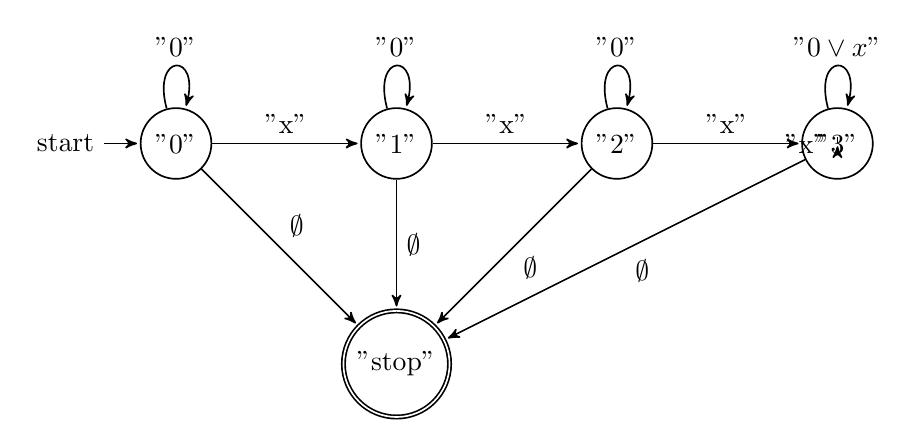
\begin{tikzpicture}[->,>=stealth',shorten >=1pt,auto,node distance=2.8cm, semithick]
\node[initial,state] (0) {"0"};
\node[state] (1) [right of=0] {"1"};
\node[state] (2) [right of=1]{"2"};
\node[state] (3) [right of=2]{"3"};
\node[accepting,state] [below of=1] (end) {"stop"};
\path (0) edge [loop above] node {"0"} (0)
(0) edge node {"x"} (1)
(0) edge node {$\emptyset$} (end)
(1) edge [loop above] node {"0"} (1)
(1) edge node {"x"} (2)
(1) edge node {$\emptyset$} (end)
(2) edge [loop above] node {"0"} (2)
(2) edge node {"x"} (3)
(2) edge node {$\emptyset$} (end)
(3) edge [loop above] node {"$0\vee x$"} (3)
(3) edge node {"x"} (3)
(3) edge node {$\emptyset$} (end);
\end{tikzpicture}
\end{center}
Insgesamt: Man kann mit endlichen Automaten nur relativ einfache Algorithmen implementieren. (nur reguläre Sprachen)
Spendiert man zusätzlichen Speicher, geht mehr:
\begin{itemize}
\item Automat mit Stack-Speicher (Stapel oder Keller) $\implies$ Kellerautomat (Kontextfreie Sprachen)
\item Automat mit zwei Stacks oder äquivalent Turing-Maschine kann alles ausführen, was man intuitiv für berechenbar hält
\end{itemize}
Markov Modelle: endliche Automaten mit probabilistischen Übergangen.
Bisher: Algorithmen für einen bestimmten Zweck (Problemklasse)
Frage: Gibt es einen universellen Algorithmus für alle berechenbare Probleme?
Betrachte formale Algorithmusbeschreibung als Teil der Eingabe des universellen Algorithmus.
\section{Substitutionsmodell (funktionale Programmierung)}
\label{sec-4}
\begin{itemize}
\item einfaches Modell für arithmetische Berechnung "Taschenrechner"
\item Eingaben und Ausgaben sind Zahlen (ganze oder reelle Zahlen). Zahlenkonstanten heißen "Literale"
\item elementare Funktionen: haben eine oder mehrere Zahlen als Argumente (Parameter) und liefern eine Zahl als Ergebnis (wie Mathematik):
\begin{itemize}
\item add(1,2) $\rightarrow$ 3, mul(2,3) $\rightarrow$ 6, analog sub(), div(), mod()
\end{itemize}
\item Funktionsaufrufe können verschachtelt werden, das heißt Argumente kann Ergebnis einer anderen Funktion sein
\begin{itemize}
\item mul(add(1,2),sub(5,3)) $\rightarrow$ 6
\end{itemize}
\end{itemize}
\subsection{Substitutionsmodell}
\label{sec-4-1}
Man kann einen Funktionsaufruf, dessen Argument bekannt ist (das heißt Zahlen sind) durch den Wert des Ergebnisses ersetzen ("substituieren"). Geschachtelte Ausdrücke lassen sich so von innen nach außen auswerten.
\[mul(add(1,2),sub(5,3))\]
\[mul(3,sub(5,3))\]
\[mul(3,2)\]
\[6\]
\begin{itemize}
\item Die arithmetischen Operationen add(), sub(), mul(), div(), mod() werden normalerweise von der Hardware implementiert.
\item Die meisten Programmiersprachen bieten außerdem algebraische Funktionen wie: sqrt(), sin(), cos(), log()
\begin{itemize}
\item sind meist nicht in Hardware, aber vorgefertigte Algorithmen, werden mit Programmiersprachen geliefert, "Standardbibliothek"
\end{itemize}
\item in C++: mathematisches Modul des Standardbibliothek: "cmath"
\item Für Arithmetik gebräuchlicher ist "Infix-Notation" mit Operator-Symbolen "+", "-", "*", "/", "\%"
\item mul(add(1,2),sub(5,3)) $\iff$ ((1+2)*(5-3))
\begin{itemize}
\item oft besser, unter anderem weil man Klammer weglassen darf
\begin{enumerate}
\item "Punkt vor Strichrechnung" 3+4*5 $\iff$ 3+(4*5), mul, div, mod binden stärker als add, sub
\item Operatoren gleicher Präzedenz werden von links nach rechts ausgeführt (links-assoziativ) \\
          1+2+3-4+5 $\iff$ ((((1+2)+3)-4)+5)
\item äußere Klammer kann man weglassen (1+2)$\iff$ 1+2
\end{enumerate}
\end{itemize}
\item Computer wandeln Infix zuerst in Präfix Notation um
\begin{enumerate}
\item weggelassene Klammer wieder einfügen
\item Operatorensymbol durch Funktionsnamen ersetzen und an Präfix-Position verschieben
\[1 + 2 + 3 * 4 / (1 + 5) - 2\]
\[(((1 + 2) + ((3 * 4) / (1 + 5))) - 2)\]
\[sub(add(add(1,2),div(mul(3,4),add(1,5))), 2)\]
\[sub(add(3,div(12,6)), 2)\]
\[sub(add(3,2), 2)\]
\[sub(5, 2)\]
\[2\]
\end{enumerate}
\end{itemize}
\subsection{Bäume}
\label{sec-4-2}
\begin{itemize}
\item bestehen aus Knoten und Kanten (Kreise und Pfeile)
\item Kanten verbinden Knoten mit ihren Kind-knoten
\item jeder Konten (außer der Wurzel) hat genau ein Elternteil ("parent node")
\item Knoten ohne Kinder heißen Blätter ("leaves / leaf node")
\item Teilbaum
\begin{itemize}
\item wähle beliebigen Knoten
\item entferne temporär dessen Elternkante, dadurch wird der Knoten temporär zu einer Wurzel, dieser Knoten mit allen Nachkommen bildet wieder einen Baum (Teilbaum des Originalbaumes)
\end{itemize}
\item trivialer Teilbaum hat nur einen Knoten
\item Tiefe: Abstand eines Knotens von der Wurzel (Anzahl der Kanten zwischen Knoten und Wurzel)
\begin{itemize}
\item Tiefe des Baums: maximale Tiefe eines Knoten
\end{itemize}
\end{itemize}
\subsubsection{Beispiel}
\label{sec-4-2-1}
\[1 + 2 + 3 * 4 / (1 + 5) - 2\]
\[sub(add(add(1,2),div(mul(3,4),add(1,5))), 2)\]
\begin{center}
\Tree [ .sub [ .add [ .add 1 2 ] [ .div [ .mul 3 4 ] [ .add 1 5 ] ] ] 2 ]
\end{center}
\subsection{Rekursion}
\label{sec-4-3}
Rekursiv $\estimates$ Algorithmus für Teilproblem von vorn.
\subsection{Präfixnotation aus dem Baum rekonstruieren}
\label{sec-4-4}
\begin{enumerate}
\item \label{algstart1} Wenn die Wurzel ein Blatt ist: Drucke die Zahl
\item sonst:
\begin{itemize}
\item Drucke Funktionsnamen
\item Drucke "("
\item Wiederhole den Algorithmus ab \ref{algstart1} für das linke Kind (Teilbaum mit Wurzel = linkes Kind)
\item Drucke ","
\item Wiederhole den Algorithmus ab \ref{algstart1} für das rechte Kind (Teilbaum mit Wurzel = rechtes Kind)
\item Drucke ")"
\end{itemize}
$\implies$ \[sub(add(add(1,2),div(mul(3,4),add(1,5))), 2)\]
\end{enumerate}
\subsection{Präfixnotation aus dem Baum rekonstruieren}
\label{sec-4-5}
\begin{enumerate}
\item \label{algstart2} Wenn die Wurzel ein Blatt ist: Drucke die Zahl
\item sonst:
\begin{itemize}
\item Drucke Funktionsnamen
\item Drucke "("
\item Wiederhole den Algorithmus ab \ref{algstart2} für das linke Kind (Teilbaum mit Wurzel = linkes Kind)
\item Drucke Operatorsymbol
\item Wiederhole den Algorithmus ab \ref{algstart2} für das rechte Kind (Teilbaum mit Wurzel = rechtes Kind)
\item Drucke ")"
\end{itemize}
$\implies$ \[sub(add(add(1,2),div(mul(3,4),add(1,5))), 2)\]
\end{enumerate}
$\implies$ \textbf{inorder}
\subsection{Berechnen des Werts mit Substitutionsmodell}
\label{sec-4-6}
\begin{enumerate}
\item \label{algstart3} Wenn Wurzel dein Blatt gib Zahl zurück
\item sonst:
\begin{itemize}
\item Wiederhole den Algorithmus ab \ref{algstart3} für das linkes Kind (Teilbaum mit Wurzel = rechtes Kind), speichere Ergebnis als "lhs"
\item Wiederhole den Algorithmus ab \ref{algstart3} für das rechte Kind (Teilbaum mit Wurzel = rechtes Kind), speichere Ergebnis als "rhs"
\item berechne funktionsname(lhs,rhs) und gebe das Ergebnis zurück
\end{itemize}
\end{enumerate}
$\implies$ \textbf{post-order}
\section{Maschinensprachen}
\label{sec-5}
\begin{itemize}
\item optimiert für die Hardware
\item Gegensatz: höhere Programmiersprachen (c++)
\begin{itemize}
\item optimiert für Programmierer
\end{itemize}
\item Compiler oder Interpreter übersetzen Hoch- in Maschinensprache
\end{itemize}
\subsection{Umwandlung in Maschinensprache}
\label{sec-5-1}
\begin{enumerate}
\item Eingaben und (Zwischen)-Ergebnisse werden in Speicherzellen abgespeichert $\implies$ jeder Knoten im Baum bekommt eine Speicherzelle
\item Speicherzellen für Eingaben initialisieren
\begin{itemize}
\item Notation: SpZ $\leftarrow$ Wert
\end{itemize}
\item Rechenoperationen in Reihenfolge des Substitutionsmodell ausführen und in der jeweiligen Speicherzelle speichern
\begin{itemize}
\item Notation: SpZ-Ergebnis $\leftarrow$ fname SpZArg1 SpZArg2
\end{itemize}
\item alles in Zahlencode umwandeln
\begin{itemize}
\item Funktionsnamen:
\begin{center}
\begin{tabular}{lr}
Opcode & Wert\\
\hline
init & 1\\
add & 2\\
sub & 3\\
mul & 4\\
div & 5\\
\end{tabular}
\end{center}
\end{itemize}
\end{enumerate}
\section{Funktionale Programmierung}
\label{sec-6}
\begin{itemize}
\item bei Maschinensprache werden Zwischenergebnisse in Speicherzellen abgelegt
\item das ist auch in der funktionalen Programmierung eine gute Idee
\item Speicherzellen werden durch Namen (vom Programmierer vergeben) unterschieden
\end{itemize}
\subsection{Beispiel}
\label{sec-6-1}
Lösen einer quadratischen Gleichung:
\[ax^2 + bx + c = 0\]
\[x^2 - 2px + q = 0, p = -\frac{b}{2a},q=\frac{c}{d}\]
\[x_2 = p + \sqrt{p^2 - q},x_2 = p - \sqrt{p^2 - q}\]
ohne Zwischenergebnisse:
\[x_1 \leftarrow add(div(div(b,a),-2),sqrt(sub(mul(div(b,a),-2),div(div(b,a)-1)),div(c,a)))\]
mit Zwischenergebnis und Infix Notation
\[p\leftarrow b / c / -2~\text{oder}~p\leftarrow -0.5 * b / a\]
\[a\leftarrow c / a\]
\[d\leftarrow sqrt(p*p - q)\]
\[x_1\leftarrow p + d\]
\[x_2\leftarrow p - d\]
\subsection{Vorteile von Zwischenergebnissen}
\label{sec-6-2}
\begin{enumerate}
\item lesbarer
\item redundante Berechnung vermieden. Beachte: In der funktionalen Programmierung können die Speicherzellen nach der Initialisierung nicht mehr verändert werden
\item Speicherzellen und Namen sind nützlich um Argumente an Funktionen zu übergeben $\implies$ Definition eigener Funktionen
\begin{minted}[tabsize=4]{cpp}
function sq(x) {
   return x * x
}
\end{minted}
$\implies$ $d \leftarrow sqrt(sq(p) - q)$
Speicherzelle mit Namen "x" für das Argument von $sq$
\end{enumerate}
\subsection{Funktionale Programmierung in c++}
\label{sec-6-3}
\begin{itemize}
\item in c++ hat jede Speicherzelle einen Typ (legt Größe und Bedeutung der Speicherzelle fest)
\begin{itemize}
\item wichtige Typen
\begin{center}
\begin{tabular}{ll}
int & ganze Zahlen\\
double & reelle Zahlen\\
std::string & Text\\
\end{tabular}
\end{center}
int: $12,-3$ \\
       double: $-1.02,1.2e-4 = 1.2*10^{-4}$ \\
       std::string: "text"
\end{itemize}
\item Initialisierung wird geschrieben als "typename spzname = Wert;"
\begin{minted}[tabsize=4]{cpp}
double a = ...;
double b = ...;
double c = ...;
double p = -0.5 b / a;
double q = c / a;
double d = std::sqrt(p*p - q);
double x1 = p + d;
double x2 = p - d;
std::cout << "x1: " << x1 << ", x2: " << x2 << std::endl;
\end{minted}
\item eigene Funktionen in C++
\begin{minted}[tabsize=4]{cpp}
// Kommentar (auch /* */)
type_ergebnis fname(type_arg1 name1, ...) {
	// Signatur / Funktionskopf / Deklaration
	return ergebnis;
	/* Funktionskörper / Definition / Implementation */
}
\end{minted}
\begin{itemize}
\item ganze Zahl quadrieren:
\begin{minted}[tabsize=4]{cpp}
int sq(int x) {
	return x*x;
}
\end{minted}
\item reelle Zahl quadrieren:
\begin{minted}[tabsize=4]{cpp}
double sq(double x) {
	return x*x;
}
\end{minted}
\item beide Varianten dürfen in c++ gleichzeitig definiert sein $\implies$ "function overloading" $\implies$ c++ wählt automatisch die richtig Variable anhand des Argumenttyps ("overload resolution")
\begin{minted}[tabsize=4]{cpp}
int x = 2;
double y = 1.1
int x2 = sq(x) // int Variante
double y2 = sq(y) // double Variante
\end{minted}
\item jedes c++-Programm muss genau eine Funktion namens "main" haben. Dort beginnt die Programmausführung.
\begin{minted}[tabsize=4]{cpp}
int main() {
	Code;
	return 0;
}
\end{minted}
\begin{itemize}
\item return aus der "main" Funktion ist optional
\end{itemize}
\item Regel von c++ für erlaubte Name
\begin{itemize}
\item erstes Zeichen: Klein- oder Großbuchstaben des englischen Alphabets, oder "\_"
\item optional: weitere Zeichen oder, "\_" oder Ziffer 0-9
\end{itemize}
\item vordefinierte Funktionen:
\begin{itemize}
\item eingebaute $\estimates$ immer vorhanden
\begin{itemize}
\item Infix-Operatoren $+,-,*,/,\%$
\item Präfix-Operatoren $operator+,operator-,\ldots$
\end{itemize}
\item Funktion der Standardbibliothek $\estimates$ müssen "angefordert" werden
\begin{itemize}
\item Namen beginnen mit "std::", "std::sin,\ldots{}"
\item sind in Module geordnet, zum Beispiel
\begin{itemize}
\item cmath $\implies$ algebraische Funktion
\item complex $\implies$ komplexe Zahlen
\item string $\implies$ Zeichenkettenverarbeitung
\end{itemize}
\item um ein Modul zu benutzen muss man zuerst (am Anfang des Programms) sein Inhaltsverzeichnis importieren (Header inkludieren) $\rightarrow$ include <name>
\begin{minted}[tabsize=4]{cpp}
#include <iostream>
#include <string>
int main() {
	std::cout << "Hello, world!" << std::endl;
	std::string out = "mein erstes Programm\n";
	std::cout << out;
	return 0;
}
\end{minted}
\end{itemize}
\end{itemize}
\item overloading der arithmetischen Operationen
\begin{itemize}
\item overloading genau wie bei $sq$
\begin{itemize}
\item 3 * 4 $\implies$ int Variante
\item 3.0 * 4.0 $\implies$ double Variante
\item 3 * 4.0 $\implies$ automatische Umwandlung in höheren Typ, hier "double" $\implies$ wird als 3.0 * 4.0 ausgeführt
\end{itemize}
\end{itemize}
\item $\implies$ Division unterscheidet sich
\begin{itemize}
\item Integer-Division: 12 / 5 = 2 (wird abgerundet)
\item Double-Division: 12.0 / 5.0 = 2.4
\item -12 / 5 = 2 ($\implies$ truncated Division)
\item 12.0 / 5.0 = 2.4
\item Gegensatz (zum Beispiel in Python)
\begin{itemize}
\item floor division $\implies$ wird immer abgerundet $\implies$ -12 / 4 = -2
\end{itemize}
\end{itemize}
\end{itemize}
\end{itemize}
\section{Prozedurale Programmierung}
\label{sec-7}
\subsection{Von der Funktionalen zur prozeduralen Programmierung}
\label{sec-7-1}
\begin{itemize}
\item Eigenschaften der Funktionalen Programmierung:
\begin{itemize}
\item alle Berechnungen durch Funktionsaufruf, Ergebnis ist Rückgabe
\item Ergebnis hängt nur von den Werten der Funktionsargumente ab, nicht von externen Faktoren "referentielle Integrität"
\item Speicherzellen für Zwischenergebnisse und Argumente können nach Initialisierung nicht geändert werden "write once"
\item Möglichkeit rekursiver Funktionsaufrufe (jeder Aufruf bekommt eigene Speicherzellen)
\begin{itemize}
\item Vorteile
\begin{itemize}
\item natürliche Ausdrucksweise für arithmetische und algebraische Funktionalität ("Taschenrechner")
\item einfache Auswertung durch Substitutionsmodell $\rightarrow$ Auswertungsreihenfolge nach Post-Order
\item mathematisch gut formalisierbar $\implies$ Korrektheitsbeweise, besonders bei Parallelverarbeitung
\item Rekursion ist mächtig und natürliche für bestimmte Probleme (Fakultät, Baum-Traversierung)
\end{itemize}
\item Nachteile
\begin{itemize}
\item viele Probleme lassen sich anders natürlicher ausdrücken (z.B. Rekursion vs. Iteration)
\item setzt unendlich viel Speicher voraus ($\implies$ Memory Management notwendig $\implies$ später)
\item Entitäten, die sich zeitlich verändern sind schwer zu modellieren
\end{itemize}
\item Korollar: kann keine externen Ressourcen (z.B. Konsole, Drucker, \ldots, Bildschirm) ansprechen "keine Seiteneffekte"
\begin{itemize}
\item $\implies$ Multi-Paradigmen-Sprachen, zum Beispiel Kombination von Funktionaler Programmierung und prozeduraler Programmierung
\end{itemize}
\end{itemize}
\end{itemize}
\end{itemize}
\subsection{Kennzeichen}
\label{sec-7-2}
\subsubsection{Prozeduren}
\label{sec-7-2-1}
\begin{itemize}
\item Prozeduren: Funktionen, die nichts zurückgeben, haben nur Seiteneffekte
\begin{itemize}
\item Beispiel
\begin{minted}[tabsize=4]{cpp}
std::cout << "Hello\n"; // Infix
operator<<(std::cout, "Hello\n"; // Präfix
\end{minted}
\item Prozeduren in c++
\begin{enumerate}
\item Funktion die "void" zurück gibt (Pseudotyp für "nichts")
\begin{minted}[tabsize=4]{cpp}
void foo(int x) {
	return;
}
\end{minted}
\item Returnwert ignorieren
\end{enumerate}
\end{itemize}
\end{itemize}
\subsubsection{Steuerung des Programmablaufs}
\label{sec-7-2-2}
\begin{itemize}
\item Anweisungen zur Steuerung des Programmablaufs
\begin{minted}[tabsize=4]{cpp}
if(), else, while(), for()
\end{minted}
\begin{itemize}
\item Funktional
\begin{minted}[tabsize=4]{cpp}
int abs(int x) {
	return (x >= 0) ? x : -x;
}
\end{minted}
\item Prozedural
\begin{minted}[tabsize=4]{cpp}
int abs(int x) {
	if(x >= 0) {
		return x;
	} else {
		return -x;
	}

	// oder
	if(x >= 0) return x;
	return -x;
}
\end{minted}
\end{itemize}
\end{itemize}
\subsubsection{Veränderung von Speicherzellen}
\label{sec-7-2-3}
\begin{itemize}
\item Zuweisung: Speicherzellen können nachträglich verändert werden ("read-write")
\begin{itemize}
\item prozedural:
\begin{minted}[tabsize=4]{cpp}
int foo(int x) {     // x = 3
	int y = 2;
	int z1 = x * y;  // z1 = 6
	y = 5;
	int z2 = z * y;  // z2 = 15
	return z1 + z2;  // 21
}
\end{minted}
\item funktional:
\begin{minted}[tabsize=4]{cpp}
int foo(int x) {      // x = 3
	int y1 = 2;
	int z1 = x * y1;  // z1 = 6
	int y2 = 5;
	int z2 = z1 * y2; // z2 = 15
	return z1 + z2;   // 21
}
\end{minted}
\item Syntax
\begin{minted}[tabsize=4]{cpp}
name = neuer_wert;           // Zuweisung
typ name = neuer_wert;       // Initialisierung
typ const name = neuer_wert; // write once
\end{minted}
\item $\implies$ Folgen: mächtiger, aber ermöglicht völlig neue Bugs $\implies$ erhöhte Aufmerksamkeit beim Programmieren
\begin{itemize}
\item die Reihenfolge der Ausführung ist viel kritischer als beim Substitutionsmodell
\item Programmierer muss immer ein mentales Bild des aktuellen Systemzustands haben
\end{itemize}
\end{itemize}
\end{itemize}
\subsubsection{Schleifen}
\label{sec-7-2-4}
Der gleiche Code soll oft wiederholt werden
\begin{minted}[tabsize=4]{cpp}
while(Bedingung) {
	// Code, wird ausgeführt solange Bedingung "true"
}
\end{minted}
\begin{minted}[tabsize=4]{cpp}
int counter = 0;
while(counter < 3) {
	std::cout << counter << std::endl;
	counter++; // Kurzform für counter = counter + 1
}
\end{minted}
\begin{center}
\begin{tabular}{rlr}
counter & Bedingung & Ausgabe\\
\hline
0 & true & 0\\
1 & true & 1\\
2 & true & 2\\
3 & false & $\emptyset$\\
\end{tabular}
\end{center}

\begin{itemize}
\item in c++ beginnt Zählung meist mit $0$ ("zero based")
\item vergisst man Inkrementieren $\implies$ Bedingung immer "true" $\implies$ Endlosschleife $\implies$ Bug
\item drei äquivalente Schreibweisen für Inkrementieren:
\begin{itemize}
\item counter = counter + 1; // assignment $\estimates$ Zuweisung
\item counter += 1;          // add-assignment $\estimates$ Abkürzung
\item ++counter;             // pre-increment
\end{itemize}
\end{itemize}
\subsubsection{prozedurale Wurzelberechnung}
\label{sec-7-2-5}
\paragraph{Ziel}
\label{sec-7-2-5-1}
\begin{minted}[tabsize=4]{cpp}
double sqrt(double y);
\end{minted}
\paragraph{Methode}
\label{sec-7-2-5-2}
iterative Verbesserung mittels Newtonverfahren
initial\_guess $x^{(0)}$ ("geraten"), t = 0 \\
     while not\_good\_enough($x^{(t)}$): \\
         update $x^{(t + 1)}$ from $x^{(t)}$ (zum Beispiel $x^{(t + 1)} = x^{(x)} + \Delta^{(t)}$ additives update, $x^{(t + 1)} = x^{(t)}\Delta^{(t)}$ multiplikatives update) \\
         t = t + 1 \\
\subparagraph{Newtonverfahren}
\label{sec-7-2-5-2-1}
Finde Nullstellen einer gegebenen Funktion $f(x)$, das heißt suche $x^\ast$ sodass $f(x^\ast) = 0$ oder $\abs{f(x^\ast)} < \varepsilon$
Taylorreihe von $f(x)$:, $f(x + \Delta) \approx f(x) + f'(x)\Delta +$ setze $x^\ast = x + \Delta$
\[0 \overset{!}{=} f(x^\ast) \approx f(x) + f'(x)\Delta = 0 \implies \Delta = - \frac{f(x)}{f'(x)}\]
Iterationsvorschrift:
\[x^{(t + 1)} = x^{(t)} - \frac{f(x^{(\ast)})}{f'(x^{(\ast)})}\]
Anwendung auf Wurzel: setze $f(x) = x^2 - y \implies$ mit $f(x^\ast) = 0$ gilt
\[(x^\ast)^2 -y = 0 \quad (x^\ast)^2 = y \quad x^\ast = \sqrt{y}\quad f'(x) = 2x)\]
Iterationsvorschrift:
\[x^{(t + 1)} = x^{(t)} - \frac{(x^{(t)^2}) - y}{2x^{(t)}} = \frac{x^{(t)^2} + y}{2x^{(t)}}\]
\begin{minted}[tabsize=4]{cpp}
double sqrt(double y) {
  if(y < 0.0) {
	  std::cout << "Wurzel aus negativer Zahl\n";
	  return -1.0;
	}
	if(y == 0.0) return 0.0;

	double x = y; // inital guess
	double epsilon = 1e-15 * y;

	while(abs(x * x - y) > epsilon) {
		x = 0.5*(x + y / x);
	}
}
\end{minted}
\subsubsection{for-Schleife}
\label{sec-7-2-6}
\begin{minted}[tabsize=4]{cpp}
int c = 0;
while(c < 3) {
	// unser Code
	c++; // vergisst man leicht
}
\end{minted}

Bei der while Schleife kann man leicht vergessen $c$ zu inkrementieren, die for Schleife ist idiotensicher \\
    Äquivalent zu der while Schleife oben ist:
\begin{minted}[tabsize=4]{cpp}
for(int c = 0; c < 3; c++) {
	// unser Code
}
\end{minted}

Allgemeine Form:
\begin{minted}[tabsize=4]{cpp}
for(init; Bedingung; Inkrement) {
	// unser Code
}
\end{minted}
\begin{itemize}
\item Befehle, um Schleifen vorzeitig abzubrechen
\begin{itemize}
\item continue: Bricht aktuelle Iteration ab und springt zum Schleifenkörper
\item break: bricht die ganze Schleife ab und springt hinter das Schleifenende
\item return: beendet Funktion und auch die Schleife
\end{itemize}
\end{itemize}
Beispiel: nur gerade Zahlen ausgeben
\begin{minted}[tabsize=4]{cpp}
for(int i = 0; i < 10; i++) if(c % 2 == 0) std::cout << c << std::endl;
\end{minted}
Variante mit continue:
\begin{minted}[tabsize=4]{cpp}
for(int i = 0; i < 10; i++) {
	if(c % 2 != 0) continue;
	std::cout << c << std::endl;
}
\end{minted}

\begin{minted}[tabsize=4]{cpp}
for(int i = 0; i < 10; i += 2) {
	std::cout << c << std::endl;
}
\end{minted}
\begin{minted}[tabsize=4]{cpp}
double sqrt(double y) {
	while(true) {
		x = (x + y / 2) / 2.0;
		if(abs(x * x - y) < epsilon) {
			return x;
		}
	}
}
\end{minted}
\section{Datentypen}
\label{sec-8}
\subsection{Basistypen}
\label{sec-8-1}
Bestandteil der Sprachsyntax und normalerweise direkt von der Hardware unterstützt (CPU)
\begin{itemize}
\item int, double, bool ($\implies$ später mehr)
\end{itemize}
\subsection{zusammengesetzte Typen}
\label{sec-8-2}
mit Hilfe von "struct" oder "class" aus einfachen Typen zusammengesetzt
\begin{itemize}
\item wie das geht $\implies$ später
\item Standardtypen: in der C++ Standardbibliothek definiert, aktivieren durch $\#include <module\_name>$
\begin{itemize}
\item std::string, std::complex, etc.
\end{itemize}
\item externe Typen: aus anderer Bibliothek, die man zuvor herunterladen und installieren muss
\item eigene Typen: vom Programmierer selbst implementiert $\implies$ später
\end{itemize}
Durch "objekt-orientierte Programmierung" ($\implies$ später) erreicht man, dass zusammengesetzte
 Typen genauso einfach und bequem und effizient sind wie Basistypen (nur c++, nicht c)
\begin{itemize}
\item "Kapselung": die interne Struktur und Implementation ist für Benutzer unsichtbar
\item Benutzer manipuliert Speicher über Funktionen ("member functions") $\estimates$ Schnittstelle des Typs, "Interface", API
\end{itemize}

$\implies$ Punktsyntax: type$\backslash$\_name t = init; t.foo(a1, a2); $\estimates$ foo(t, a1, a2);
\subsection{Zeichenketten-Strings:}
\label{sec-8-3}
zwei Datentypen in c++
\begin{itemize}
\item klassischer c-string: char[] ("Charakter Array") $\implies$ nicht gekapselt, umständlich
\item c++ string: std::string gekapselt und bequem (nur dieser in der Vorlesung)
\item string Literale: "Zeichenkette", einzelnes Zeichen: 'z' ("z" = Kette der Länge 1) \\
     Vorsicht: die String-Literale sind c-strings (gibt keine c++ string-Literale),
müssen erst in c++ strings umgewandelt werden, das passiert meist automatisch
\begin{itemize}
\item \#include <string>
\item Initialisierung:
\begin{minted}[tabsize=4]{cpp}
std::string s = "abcde";
std::string s2 = s1;
std::string leer = "";
std::string leer(); // Abkürzung, default Konstruktor
\end{minted}
\item Länge
\begin{minted}[tabsize=4]{cpp}
s.size();
assert(s.size() == 5);
assert(leer.size() == 0);
s.empty() // Abkürzung für s.size() == 0
\end{minted}
\item Zuweisung
\begin{minted}[tabsize=4]{cpp}
s = "xy";
s2 = leer;
\end{minted}
\item Addition
Aneinanderkettung von String ("concatenate")
\begin{minted}[tabsize=4]{cpp}
std::string s3 = s + "ijh"; // "xyijh"
s3 = "ghi" + s; // "ghixy"
s3 = s + s; // "xyxy"
// aber nicht!!
s3 = "abc" + "def"; // Bug Literale unterstützen + mit ganz anderer Bedeutung
s3 = std::string("abc") + "def"; // Ok
\end{minted}
\item Add-Assignment: Abkürzung für Addition gefolgt von Zuweisung
\begin{minted}[tabsize=4]{cpp}
s += "nmk"; // s = s + "nmk" => "xynmk"
\end{minted}
\item die Zeichen werden intern in einem C-Array gespeichert (Array = "Feld") \\
       Array: zusammenhängende Folge von Speicherzellen des gleichen Typs, hier 'char' (für einzelne Zeichen), Die Länge wird (bei std::string) automatisch angepasst, die einzelnen Speicherzellen sind durchnummeriert
in c++: von $0$ beginnend $\estimates$ Index
\begin{itemize}
\item Indexoperator:
\begin{minted}[tabsize=4]{cpp}
s[index]; // gibt das Zeichen an Position "index" zurück
\end{minted}
Anwendung: jedes Zeichen einzeln ausgeben
\begin{minted}[tabsize=4]{cpp}
std::string s = "abcde";

for(int i = 0; i < s.size(); i++) {
	std::cout << s[i] << std::endl;
}
\end{minted}
String umkehren
\begin{minted}[tabsize=4]{cpp}
int i = 0; // Anfang des Strings
int k = s.size() - 1; // Ende des String
while(i < k) {
	char tmp = s[i];
	s[i] = s[k];
	s[k] = tmp;
	i++; k--;
}
\end{minted}
Variante 2: neuen String erzeugen
\begin{minted}[tabsize=4]{cpp}
std::string s = "abcde";
std::string r = "";
for(int i = s.size() - 1; i >= 0; i--) {
	r += s[i];
}
\end{minted}
\end{itemize}
\end{itemize}
\end{itemize}
\section{Umgebungsmodell}
\label{sec-9}
Gegenstück zum Substitutionsmodell (in der funktionalen Programmierung) für die prozedurale Programmierung
\begin{itemize}
\item Regeln für Auswertung von Ausdrücken
\item Regeln für automatische Speicherverwaltung
\begin{itemize}
\item Freigeben nicht mehr benötigter Speicherzellen, $\implies$ bessere Approximation von "unendlich viel Speicher"
\end{itemize}
\item Umgebung beginnt normalerweise bei "\{" und endet bei "\}" \\
    Ausnahmen:
\begin{itemize}
\item $for$: Umgebung beginnt schon bei "for" $\implies$ Laufvariable ist Teil der Umgebung
\item Funktionsdefinitionen: Umgebung beginnt beim Funktionskopf $\implies$ Speicherzellen für Argumente und Ergebnis gehören zur Umgebung
\item globale Umgebung außerhalb aller "\{ \}" Klammern
\end{itemize}
\item automatische Speicherverwaltung
\begin{itemize}
\item Speicherzellen, die in einer Umgebung angelegt werde (initialisiert, deklariert) werde, am Ende der Umgebung in umgekehrter Reihenfolge freigegeben
\item Computer fügt vor "\}" automatisch die Notwendigen Befehle ein
\item Speicherzellen in der globalen Umgebung werden am Programmende freigegeben
\begin{minted}[tabsize=4]{cpp}
- int global = 1;
  int main() {
	  int l = 2;
	  {
		  int m = 3
	  } // <- m wird freigegeben
  } // <- l wird freigegeben
  // <- global wird freigegeben
\end{minted}
\end{itemize}
\item Umgebungen können beliebig geschachtelt werden $\implies$ alle Umgebungen bilden einen Baum, mit der globalen Umgebung als Wurzel
\item Funktionen sind in der globalen Umgebung definiert
\begin{itemize}
\item Umgebung jeder Funktion sind Kindknoten der globalen Umgebung (Ausnahme: Namensräume $\implies$ siehe unten) \\
      $\implies$ Funktions Umgebung ist \textbf{nicht} in der Umgebung, wo die Funktion aufgerufen wird
\end{itemize}
\item Jede Umgebung besitzt eine \textbf{Zuordnungstabelle} für alle Speicherzellen, die in der Umgebung definiert wurden
\begin{center}
\begin{tabular}{llr}
Name & Typ & aktueller Wert\\
\hline
l & int & 2\\
\end{tabular}
\end{center}
\item jeder Name kann pro Umgebung nur einmal vorkommen
\item Ausnahme Funktionsnamen können mehrmals vorkommen bei function overloading (nur c++)
\item Alle Befehle werden relativ zur aktuellen Umgebung ausgeführt
\begin{itemize}
\item aktuell: Zuordnungstabelle der gleichen Umgebung und aktueller Wert zum Zeitpunkt des Aufrufs \\
      Beispiel: $c = a * b;$ \\
      Regeln:
\item wird der Name (nur $a, b, c$) in der aktuellen Zuordnungstabelle gefunden
\begin{enumerate}
\item Typprüfung $\implies$ Fehlermeldung, wenn Typ und Operation nicht zusammenpassen
\item andernfalls, setze aktuellen Wert aus Tabelle in Ausdruck ein (ähnlich Substitutionsmodell)
\end{enumerate}
\item wird Name nicht gefunden: suche in der Elternumgebung weiter
\item wird der Name bis zur Wurzel (globale Umgebung) nicht gefunden $\implies$ Fehlermeldung
\item $\implies$ ist der Name in mehreren Umgebungen vorhanden gilt der zuerst gefundene (Typ, Wert)
\end{itemize}
\item $\implies$ Programmierer muss selbst darauf achten, dass
\begin{enumerate}
\item bei der Suche die gewünschte Speicherzelle gefunden wird $\implies$ benutze "sprechende Namen"
\item der aktuelle Wert der richtig ist $\implies$ beachte Reihenfolge der Befehle!
\end{enumerate}
\item Namensraum: spezielle Umgebungen in der globalen Umgebung (auch geschachtelt) mit einem Namen \\
    Ziele:
\begin{itemize}
\item Gruppieren von Funktionalität in Module (zusätzlich zu Headern)
\item Verhinderung von Namenskollisionen
\end{itemize}
Beispiel: c++ Standardbibliothek:
\begin{minted}[tabsize=4]{cpp}
namespace std {
double sqrt(double x);
namespace chrono {
class system_clock;
}
}

// Benutzung mit Namespace-Präfix:
std::sqrt(80);
std::chrono::system_clock clock;
\end{minted}
 Besonderheit: mehrere Blöcke mit selbem Namensraum werden verschmolzen
Beispiel
\begin{minted}[tabsize=4]{cpp}
int p = 2;
int q = 3;

int foo(int p) {
	return p * q;
}

int main() {
	int k = p * q; // beides global => 6 = 2 * 3
	int p = 4; // lokales p verdeckt globales p
	int r = p * q; // p lokal, q global => 12 = 4 * 3
	int s = foo(p); // lokale p von main() wird zum lokalen p von foo() 12 = 4 * 3
	int t = foo(q); // globales q wird zum lokalen p von foo() 9 = 3 * 3
	int q = 5;
	int n = foo(g); // lokales q wird zum lokalen p von foo() 15 = 5 * 3
}
\end{minted}
\end{itemize}
\section{Referenzen}
\label{sec-10}
sind neue (zusätzliche) Namen für vorhandene Speicherzellen
\begin{minted}[tabsize=4]{cpp}
int x = 3; // neue Variable x mit neuer Speicherzelle
int & y = x; // Referenz: y ist neuer Name für x, beide haben die selbe Speicherzelle
y = 4; // Zuweisung an y, aber x ändert sich auch, das heißt x == 4
x = 5; // jetzt y == 5
int const & z = x; // read-only Referenz, das heißt z = 6 ist verboten
x = 6; // jetzt auch z == 6
\end{minted}
Hauptanwendung:
\begin{itemize}
\item die Umgebung, in der eine Funktion aufgerufen wird und die Umgebung der Implementation sind unabhängig, das heißt Variablen der einen Umgebung sind in der anderen nicht sichtbar
\item häufig möchte man Speicherzellen in beiden Umgebungen teilen $\implies$ verwende Referenzen
\item häufig will man vermeiden, dass eine Variable kopiert wird (pass-by-value)
\begin{itemize}
\item Durch pass-by-reference braucht man keine Kopie $\implies$ typisch "const \&", also read-only, keine Seiteneffekte
\begin{minted}[tabsize=4]{cpp}
int foo(int x) { // pass-by-value
	x += 3;
	return x;
}

int bar(int & y) { // pass-by-reference
	y += 3; // Seiteneffekt der Funktion
	return y;
}

void baz(int & z) { // pass-by-reference
	z += 3;
}

int main() {
	int a = 3;
	std::cout << foo(a) << std::endl; // 5
	std::cout << a << std::endl; // 3
	std::cout << bar(a) << std::endl; // 5
	std::cout << a << std::endl; // 5
	baz(a);
	std::cout << a << std::endl; // 8
}
\end{minted}
in der funktionalen Programmierung sind Seiteneffekte grundsätzlich verboten, 
mit Ausnahmen, zum Beispiel für Ein-/Ausgabe
\end{itemize}
\end{itemize}
\section{Container-Datentypen}
\label{sec-11}
Dienen dazu, andere Daten aufzubewahren
\begin{itemize}
\item Art der Elemente:
\begin{itemize}
\item homogene Container: alle Elemente haben gleichen Type (typisch für c++)
\item heterogene Container: Elemente könne verschiedene Typen haben (z.B. Python)
\end{itemize}
\item nach Größen
\begin{itemize}
\item statische Container: feste Größe, zur Compilezeit bekannt
\item dynamische Container: Größe zur Laufzeit veränderbar
\end{itemize}
\item Arrays sind die wichtigsten Container, weil effizient auf Hardware abgebildet und einfach zu benutzen
\begin{itemize}
\item klassisch: Arrays sind statisch, zum Beispiel C-Arrays (hat c++ geerbt)
\begin{minted}[tabsize=4]{cpp}
int a[20];
\end{minted}
\item modern: dynamische Arrays
\begin{itemize}
\item Entdeckung einer effizienten Implementation
\item Kapselung durch objekt-orientierte Programmierung (sonst zu kompliziert)
\end{itemize}
\end{itemize}
\item wir kennen bereits ein dynamisches Array: std::string ist Abbildung int (Index) $\rightarrow$ char (Zeichen), mit $0 \leq~\text{index}~ < ~\text{s.size()}$
\begin{itemize}
\item wichtigste Funktion: s.size() (weil Größe dynamisch), s[4 ] Indexzugriff, s+="mehr" Zeichen anhängen
\end{itemize}
\item wir wollen dasselbe Verhalten für beliebige Elementtypen:
\begin{minted}[tabsize=4]{cpp}
#include <vector>

//          Elementtyp    Größe  Initialwert der Elemente
std::vector<double    > v(20   ,           0.0           );
// analog
std::vector<int>;
std::vector<std::string>;
\end{minted}
\item weitere Verallgemeinerung: Indextyp beliebig (man sagt dann "Schlüssel-Typ") "assoziatives Array"
\begin{itemize}
\item typische Fälle:
\begin{itemize}
\item Index ist nicht im Bereich (0,size], zum Beispiel Matrikelnummern
\item Index ist string, zum Beispiel Name eines Studenten
\begin{minted}[tabsize=4]{cpp}
#include <map>
#include <unordered_map>

// Binärer Suchbaum
std::map;

// Hashtabelle, siehe Algorithmen und Datenstrukturen
std::unordered_map;

//       Schlüsseltyp  Elementtyp
std::map<int         , double> noten; noten[3121101] = 10;
std::map<std::string, double> noten; noten["krause"] = 10;
\end{minted}
\item Indexoperationen wie beim Array
\item Elemente werden beim 1. Zugriff automatisch erzeugt (dynamisch)
\end{itemize}
\end{itemize}
\item alle dynamischen und assoziativen Arrays unterstützen a.size() zum Abfragen der Größe
\end{itemize}
\subsection{std::vector}
\label{sec-11-1}
\begin{itemize}
\item Erzeugen:
\begin{minted}[tabsize=4]{cpp}
std::vector<double> v(20, 1.0);
std::vector<double> v; // leeres Array
std::vector<double> v = {1.0, -3.0, 2.2}; // "initializer list": Element für Anfangszustand
\end{minted}
\item Größe:
\begin{minted}[tabsize=4]{cpp}
v.size();
v.empty(); // => v.size() == 0
\end{minted}
\item Größe ändern
\begin{minted}[tabsize=4]{cpp}
v.resize(neue_groesse, initialwert);
// Dann:
// Fall 1: neue_groesse < size(): Element ab Index "neue_groesse" gelöscht die andern bleiben
// Fall 2: neue_groesse > size(): neue Elemente mit Initialwert am Ende anhängen, die anderen bleiben
// Fall 3: neue_groesse == size(): nichts passiert

v.push_back(neues_element); // ein neues Element am Ende anhängen (ähnlich string += "mehr")
v.insert(v.begin() + index, neues_element); // neues element an Position "index" einfügen 0 <= index <= size()
// Falls index == size(): am Ende anhängen, sonst: alte Elemente ab Index werden eine Position nach hinten verschoben (teuer)

v.pop_back(); // letztes Element löschen (effizient)
v.erase(v.begin() + index); // Element an Position index löschen, alles dahinter eine Position verschieben (teuer)
v.clear(); // alles löschen
\end{minted}
\item Zugriff
\begin{minted}[tabsize=4]{cpp}
v[k]; // Element bei Index k
v.at(k); // wie v[k], aber Fehlermeldung, wenn nicht 0 <= k < size() (zum Debuggen)
\end{minted}
\item Funktionen für Container benutzen in c++ immer Iteratoren, damit sie für verschiedene Container funktionieren
\begin{itemize}
\item Iterator-Range
\begin{minted}[tabsize=4]{cpp}
// erstes Element
v.begin()

// hinter letztem Element
v.end()
\end{minted}
\item im Header <algorithm>
\item alle Elemente kopieren
\begin{minted}[tabsize=4]{cpp}
std::vector<double> source = {1.0, 2, 3, 4, 5};
std::vector<double> target(source.size(), 0.0);
std::copy(source.begin(), source.end(), target.begin());
std::copy(source.begin() + 2, source.end() - 1, target.begin()); // nur index 2 .. size() - 1 kopieren
\end{minted}
\item Elemente sortieren
\begin{minted}[tabsize=4]{cpp}
std::sort(v.begin(), v.end()); // "in-place" sortieren
\end{minted}
\item Elemente mischen:
\begin{minted}[tabsize=4]{cpp}
std::random_shuffle(v.begin(), v.end()); // "in-place" mischen
\end{minted}
\end{itemize}
\end{itemize}
\subsubsection{Effizienz von push$\backslash$\_back}
\label{sec-11-1-1}
Warum ist push$\backslash$\_back() effizient? (bei std::vector)
\begin{itemize}
\item veraltete Lehrmeinung: Arrays sind nur effizient wenn statisch (das heißt Größe zur Compilezeit, oder spätestens bei Initialisierung, bekannt)
\begin{itemize}
\item sonst: andere Datenstruktur verwenden, zum Beispiel verkettete Liste (std::list)
\end{itemize}
\item modern: bei vielen Anwendungen genügt, wenn Array (meist) nur am Ende vergrößert wird (zum Beispiel push\_back())
\begin{itemize}
\item dies kann sehr effizient unterstützt werden $\implies$ dynamisches Array
\end{itemize}
\item std::vector verwaltet intern ein statisches Array der Größe "capacity", v.capacity() >= c.size()
\begin{itemize}
\item wird das interne Array zu klein $\implies$ wird automatisch auf ein doppelt so großes umgeschaltet
\item ist das interne Array zu groß, bleiben unbenutzte Speicherzellen als Reserve
\end{itemize}
\item Verhalten bei push$\backslash$\_back():
\begin{enumerate}
\item noch Reserve vorhanden: lege neues Element im eine unbenutzte Speicherzelle $\implies$ billig
\item keine Reserve
\begin{enumerate}
\item alloziere neues statisches Array mit doppelt Kapazität
\item kopiere die Daten aus dem altem in das neue Array
\item gebe das alte Array frei
\item gehe zum Anfang des Algorithmus, jetzt ist wieder Reserve vorhanden
\end{enumerate}
\end{enumerate}
\item das Umkopieren ist nicht zu teuer, weil es nur selten notwendig ist
\item Beispiel:
\begin{minted}[tabsize=4]{cpp}
std::vector<int> v;

for(int i = 0; i < 32; i++) v.push_back(k);
\end{minted}
\begin{center}
\begin{tabular}{rrrrrr}
k & capacity vor push\_back() & capacity nach push\_back() & size() & Reserve & \#Umkopieren\\
\hline
0 & 0 & 1 & 1 & 0 & 0\\
1 & 1 & 2 & 2 & 0 & 1\\
\hline
2 & 2 & 4 & 3 & 1 & 2\\
3 & 4 & 4 & 4 & 0 & 2\\
\hline
4 & 4 & 8 & 5 & 3 & 4\\
5-7 & 8 & 8 & 8 & 0 & 0\\
\hline
8 & 8 & 16 & 9 & 7 & 8\\
9-15 & 16 & 16 & 16 & 0 & 0\\
\hline
16 & 16 & 32 & 17 & 15 & 16\\
17-31 & 32 & 32 & 32 & 0 & 0\\
\end{tabular}
\end{center}
\begin{itemize}
\item was kostet das:
\begin{itemize}
\item 32 Elemente einfügen = 32 Kopien extern $\implies$ intern
\item aus allem Array ins neu kopieren $(1 + 2 + 4 + 8 + 16) = 31$ kopieren intern $\implies$ intern
\item $\implies$ im Durchschnitt sind pro Einfügung 2 Kopien nötig
\item $\implies$ dynamisches Array ist doppelt so teuer sie das statische  $\implies$ immer noch sehr effizient
\end{itemize}
\end{itemize}
\item relevante Funktionen von std::vector
\begin{minted}[tabsize=4]{cpp}
v.size() // aktuelle Zahl der Elemente
v.capacity() // aktuelle Zahl Speicherzellen
assert(v.capacity() - v.size() >= 0) // Reserve
v.resize(new_size) // ändert immer v.size(), aber v.capacity() nur wenn < new_size
v.reserve(new_capacity) // ändert v.size() nicht, aber v.capacity() falls new_capacity >= size
v.shrink_to_fit() // == v.reserve/v.size()) Reserve ist danach 0, wenn Endgröße erreicht
\end{minted}
\item wenn Reserve > size: capacity kann auch halbiert werden
\item wichtige Container der c++ Standardbibliothek
\item wir hatten dynamische Arrays std::string, std::vector, assoziative Arrays std::map, std::unordered$\backslash$\_map
\item std::set, std::unordered$\backslash$\_set: Menge, jedes Element ist höchstens einmal enthalten zum Beispiel Duplikate
\item std::stack (Stapel, Keller): unterstützt push und pop() mit Last in- First out Semantik (LIFO) äquivalent zu push\_back() und pop\_back() bei std::vector
\item std::queue (Warteschlange) push() und pop() mit First in-first out Semantik (FIFO)
\item std::deque ("double-ended queue") gleichzeitig stack und queue, push, pop$\backslash$\_front(), pop$\backslash$\_back()
\item std::priority$\backslash$\_queue, push() und pop() - Element mit höchster niedrigster Priorität (user defined)
\end{itemize}
\section{Iteratoren}
\label{sec-12}
\begin{itemize}
\item für Arrays lautet die kanonische Schleife
\begin{minted}[tabsize=4]{cpp}
for(int i = 0; i != v.size(); i++) {
	int current = v[i]; // lesen
	v[i] = new_value; // schreiben
}
\end{minted}
\item wir wollen eine so einfache Schleife für beliebige Container
\begin{itemize}
\item der Index-Zugriff v[] ist bei den meisten Container nicht effizient
\item Iteratoren sind immer effizient $\implies$ es gibt sie in allen modernen Programmiersprachen, aber Details sehr unterschiedlich
\item Analogie: Zeiger einer Uhr, Cursor in Textverarbeitung
\begin{itemize}
\item $\implies$ ein Iterator zeigt immer auf ein Element des Containers, oder auf Spezialwert "ungültiges Element"
\end{itemize}
\item in c++ unterstützt jeder Iterator 5 Grundoperationen
\begin{enumerate}
\item Iterator auf erstes Element erzeugen: auto iter = v.begin();
\item Iterator auf "ungültiges Element" erzeugen: auto end = v.end();
\item Vergleich $iter1 == iter2$ (Zeigen auf gleiches Element), $iter != end$:
\end{enumerate}
iter zeigt \textbf{nicht} auf ungültiges Element
\begin{enumerate}
\item zum nächsten weitergehen: ++iter. Ergebnis ist v.end(), wenn man vorher beim letzten Element war
\item auf Daten zugreifen: *iter ("Dereferenzierung") analog v[k]
\end{enumerate}
kanonische Schleife:
\begin{minted}[tabsize=4]{cpp}
for(auto iter = v.begin(); iter != v.end(); ++iter) {
int current = *iter; // lesen
*iter = new_value; // schreiben
}
// Abkürzung: range-based for loop
for(auto & element : v) {
int current = element; // lesen
element  = new_value; // schreiben
}
\end{minted}
\end{itemize}
\item Iteratoren mit den 5 Grundoperationen heißen "forward iterator" (wegen ++iter)
\item "bidirectional iterators": unterstützen auch $--iter$, zum vorigen Element ((fast) alle Iteratoren in std)
\item "random access iterators": beliebige Sprünge "iter += 5; iter -= 3;"
\item Besonderheit für assoziative Arrays (std::map, std::unordered$\backslash$\_map)
Schlüssel und Werte können beliebig gewählt werden
\begin{itemize}
\item $\implies$ das aktuelle Element ist ein Schlüssel / Wert -Paar, das heißt Iterator gibt Schlüssel und Wert zurück
\begin{minted}[tabsize=4]{cpp}
(*iter).first; // Schlüssel
(*iter).second; // Wert
// Abkürzung
iter->first;
iter->second;
\end{minted}
\begin{itemize}
\item bei std::map liefern die Iteratoren die Elemente in aufsteigender Reihenfolge der Schlüssel
\end{itemize}
\end{itemize}
\item Die Funktion std::transform()
\begin{itemize}
\item wir hatten: std::copy()
\begin{minted}[tabsize=4]{cpp}
std::vector<double> source = {1, 2, 3, 4};
std::vector<double> target(source.size());
std::copy(source.begin(), source.end(), target.begin());
\end{minted}
\item std::transform:
\begin{minted}[tabsize=4]{cpp}
// nach Kleinbuchstaben konvertieren
std::string source = "aAbCdE";
std::string target = source;
std::transform(source.begin(), source.end(), target.begin(), std::tolower); // Name einer Funktion, die ein einzelnes Element transformiert, t="aabcde"
// die Daten quadrieren
double sq(double x) { return x * x; }
std::transform(source.begin(), source.end(), target.begin(), sq); // target == {1, 4, 9, 16}
// das ist eine Abkürzung für eine Schleife
auto src_begin = source.begin();
auto src_end = source.end();
auto tgt_begin = target.begin();

for(; src_begin != src_end; src_begin++, tgt_begin++) {
	*tgt_begin = sq(*src_begin);
}
\end{minted}
\begin{itemize}
\item Der Argumenttyp der Funktion muss mit dem source Elementtyp kompatibel sein. Der Returntyp der Funktion muss mit dem Target-Elementtyp kompatibel sein.
\item Das letzte Argument von std::transform() muss ein Funktor sein (verhält sich wie eine Funktion), drei Varianten:
\begin{enumerate}
\item normale Funktion, z.B. sq. Aber: wenn Funktion für mehrere Argumenttypen überladen ist (overloading) (zum Beispiel, wenn es sq(double) und sq(int) gibt), muss der Programmierer dem Compiler sagen, welche Version gemeint ist $\implies$ für Fortgeschrittene ("functionpointer cast")
\item Funktionsobjekt $\implies$ objekt-orientierte Programmierung
\item Definiere eine namenlose Funktion $\implies$ "Lambda-Funktion $\lambda$"
\begin{itemize}
\item statt $\lambda$ verwenden wir den Universalnamen []
\begin{minted}[tabsize=4]{cpp}
std::transform(source.begin(), source.end(), target.begin(), [](double x) { return x*x; }); // statt Funktionsname sq wie bei 1 steht hier die ganz Funktionsimplementation
// Returntyp setzt Computer automatisch ein, wenn es nur einen return-Befehl gibt.
\end{minted}
\item Lambda-Funktionen können noch viel mehr $\implies$ für Fortgeschrittene
\item std::transform() kann in-place arbeiten (das heißt source-Container überschreiben), wenn source und target gleich
\begin{minted}[tabsize=4]{cpp}
std::transform(source.begin(), source.end(), source.begin(), sq);
\end{minted}
\end{itemize}
\end{enumerate}
\item Die Funktion std::sort() zum in-place sortieren eines Arrays
\begin{minted}[tabsize=4]{cpp}
std::vector<double> v = {4, 2, 3, 5 ,1};
std::sort(v.begin(), v.end()); // v == {1, 2, 3, 4, 5}
\end{minted}
\item std::sort ruft intern den $<$-Operator des Elementtyps auf, um Reihenfolge zu bestimmen
\item die $<$-Operation muss eine totale Ordnung der Elemente definieren:
\begin{itemize}
\item $a < b$ muss für beliebige $a,b$ ausführbar sein
\item transitiv: $(a < b) \wedge (b < c) \implies (a < c)$
\item anti-symmetrisch: $\neg(a < b) \wedge \neg(b < a) \implies a == b$
\end{itemize}
\end{itemize}
\end{itemize}
\end{itemize}

\section{Insertion Sort}
\label{sec-13}
schnellster Sortieralgorithmus für kleine Arrays ($n\leq 30$) hängt von Compiler und CPU ab
\begin{itemize}
\item Idee von Insertion Sort:
\begin{itemize}
\item wie beim Aufnehmen und Ordnen eines Kartenblatts
\item gegeben: bereits sortierte Teilmenge bis Position $k - 1$ Karten bereits in Fächer
\item Einfügen des k-ten Elements an richtiger Stelle $\rightarrow$ Erzeuge Lücke an richtiger Position durch verschieben von Elementen nach rechts
\item Wiederholung für $k = 1, \ldots, N$
\item Beispiel:
\begin{center}
\begin{tabular}{rrrrr}
4 & 2 & 3 & 5 & 1\\
\hline
4 & \_ & 3 & 5 & 1\\
\_ & 4 & 3 & 5 & 1\\
2 & 4 & 3 & 5 & 1\\
\hline
2 & 4 & \_ & 5 & 1\\
2 & \_ & 4 & 5 & 1\\
2 & 3 & 4 & 5 & 1\\
\hline
2 & 3 & 4 & \_ & 1\\
2 & 3 & 4 & 5 & 1\\
\hline
2 & 3 & 4 & 5 & \_\\
\_ & 2 & 3 & 4 & 5\\
1 & 2 & 3 & 4 & 5\\
\end{tabular}
\end{center}
\begin{minted}[tabsize=4]{cpp}
void insertion_sort(std::vector<double> & v) {
	for(int i = 0; i < v.size(); i++) {
		double current = v[i];
		int j = i; // Anfangsposition der Lücke
		while(j > 0) {
			if(v[j - 1] < current) { // -> if(cmp(a, b))
				break; // j ist richtige Position der Lücke
			}
			v[j] = v[j - 1];
			j--;
		}
		v[j] = current;
	}
}
\end{minted}
\item andere Sortierung: definiere Funktor cmp(a, b), der das gewünschte kleiner realisiert (gibt genau dann "true" zurück, wenn a "kleiner" b nach neuer Sortierung)
\item neue Sortierung am besten per Lambda-Funktion an std::sort übergeben
\begin{minted}[tabsize=4]{cpp}
std::sort(v.begin(), v.end()); // Standartsort mit "<"
std::sort(v.begin(), v.end(), [](double a, double b) { return a < b; }); // Standardsortierung aufsteigen
std::sort(v.begin(), v.end(), [](double a, double b) { return b < a; }); // absteigende Sortierung
std::sort(v.begin(), v.end(), [](double a, double b) { return std::abs(a) < std::abs(b); }); // Normal nach Betrag; // Normal nach Betrag
std::sort(v.begin(), v.end(), [](std::string a, std::string b) {
	std::transform(a.begin(), a.end(), a.begin(), std::tolower);
	std::transform(b.begin(), b.end(), b.begin(), std::tolower);
	return a < b;
});
\end{minted}
\end{itemize}
\end{itemize}
\section{generische Programmierung}
\label{sec-14}
insertion$\backslash$\_sort soll für beliebige Elementtypen funktionieren
\begin{minted}[tabsize=4]{cpp}
template<typename T>
void insertion_sort(std::vector<T> & v) {
	for(int i = 0; i < v.size(); i++) {
		T current = v[i];
		int j = i; // Anfangsposition der Lücke
		while(j > 0) {
			if(v[j - 1] < current) { // -> if(cmp(a, b))
				break; // j ist richtige Position der Lücke
			}
			v[j] = v[j - 1];
			j--;
		}
		v[j] = current;
	}
}
\end{minted}
\begin{itemize}
\item Ziel: benutze template-Mechanismus, damit \textbf{eine} Implementation für viele verschiedene Typen verwendbar ist
\begin{itemize}
\item erweitert funktionale und prozedurale und objekt-orientiere Programmierung
\end{itemize}
\item zwei Arten von Templates ("Schablone"):
\begin{enumerate}
\item Klassen-templates für Datenstrukturen, zum Beispiel Container sollen beliebige Elementtypen unterstützen
\begin{itemize}
\item Implementation $\implies$ später
\item Benutzung: Datenstrukturname gefolgt vom Elementtyp in spitzen Klammern (std::vector<double>), oder mehrere Typen, zum Beispiel Schlüssel und Wert bei std::map<std::string, double>
\end{itemize}
\item Funktionen-Templates: es gab schon function overloading
\begin{minted}[tabsize=4]{cpp}
int sq(int x) {
	return x * x;
}

double sq(double x) {
   return x * x;
}

// und so weiter für komplexe und rationale Zahlen...
\end{minted}
\begin{itemize}
\item Nachteil
\begin{itemize}
\item wenn die Implementationen gleich sind $\rightarrow$ nutzlose Arbeit
\item Redundanz ist gefährlich: korrigiert man einen Bug wir leicht eine Variante vergessen
\end{itemize}
\item mit templates reicht eine Implementation
\begin{minted}[tabsize=4]{cpp}
template<typename T> // T: Platzhalter für beliebigen Typ, wird später durch einen tatsächlichen Typ ersetzt
T sq(T x) {
	return x * x; // implizierte Anforderung an den Typ T, er muss Multiplikation unterstützen, sonst: Fehlermeldung
}
\end{minted}
\begin{itemize}
\item wie bei Substituieren von Variablen mit Werten, aber jetzt mit Typen
\item Benutzung:
\begin{itemize}
\item Typen für die Platzhalter hinter dem Funktionsnamen in spitzen klammern
\begin{minted}[tabsize=4]{cpp}
sq<int>(2) == 4;
sq<double>(3.0) == 9.0,
\end{minted}
\item meist kann man die Typenangabe <type> weglassen, weil der Computer sie anhand des Argumenttyps automatisch einsetzt:
\begin{minted}[tabsize=4]{cpp}
sq(2); // == sq<int>(2) == 4
sq(3.0); // == sq<double>(3.0) == 9
\end{minted}
\item kombiniert man templates mit Overloading, wird die ausprogrammierte Variante vom Compiler bevorzugt.
Komplizierte Fälle (Argument teilweise Template, teilweise hard\_coded) $\implies$ für Fortgeschrittene
\end{itemize}
\item Beispiel 2: Funktion, die ein Array auf Konsole ausgibt, für beliebige Elementtypen
\begin{minted}[tabsize=4]{cpp}
template<typename ElementType>
void print_vector(std::vector<ElementType> const & v) {
	std::cout << "{";
	if(v.size() > 0) {
		std::cout << " " << v[0];
		for(int i = 1; i < v.size(); i++) {
			std::cout << ", " << v[i];
		}
	}
	std::cout << " }";
}
\end{minted}
\item Verallgemeinerung für beliebige Container mittels Iteratoren:
\begin{minted}[tabsize=4]{cpp}
std::list<int> l = {1, 2, 3};
print_container(l.begin(), l.end()); // "{1,2,3}"
\end{minted}
\item es genügen forward\_itertators
\begin{minted}[tabsize=4]{cpp}
Iterator iter2 = iter1; // Kopie erzeugen
iter1++; // zum nächsten Element
iter1 == iter2; // Zeigen sie auf das selbe Element?
iter1 != end;
*iter1; // Zugriff auf aktuelles Element

template<typename Iterator>
void print_container(Iterator begin, Iterator end) {
	std::cout << "{}";
	if(begin != end) { // Container nicht leer?
		std::cout << " " << *begin++;
		for(;begin != end; begin++) {
			std::cout << ", " << *begin;
		}
	std::cout << "}";
}
\end{minted}
\item Beispiel 3: überprüfen, ob Container sortiert ist
\begin{minted}[tabsize=4]{cpp}
template<typename E, typename CMP>
bool check_sorted(std::vector<E> const & v, CMP less_than) {
	for(int i = 1; i < v.size(); i++) {
		if(less_than(v[k], v[k - 1])) { // statt v[k] < v[k - 1], ausnutzen der Transitivität
			return false;
		}
	}
	return true;
}

// Aufruf:
std::vector<double> v = {1.0, 2.0, 3.0};
check_sorted(v, [](double a, double b) { return a < b; } ); // == true

check_sorted(v, [](double a, double b) { return a > b; } ); // == false

// Implementation für Iteratoren
template<typename Iterator, typename CMP>
bool check_sorted(Iterator begin, Iterator end, CMP less_than) {
	if(begin == end) {
		return true;
	}
	Iterator next = begin;
	++next;
	for(; next != end; ++begin, ++next) {
		if(less_than(*next, *begin)) {
			return false;
		}
	}
	return true;
}
// == std::is_sorted
\end{minted}
\item Bemerkung: Compiler-Fehlermeldungen bei Template-Code sind oft schwer zu interpretieren, $\implies$ Erfahrung nötig aber: Compiler werden darin immer besser, besonders clang-Compiler
\item mit Templates kann man noch viel raffinierter Dinge machen, zum Beispiel Traits-Klassen, intelligent libraries template meta programming $\implies$ nur für Fortgeschrittene
\end{itemize}
\end{itemize}
\end{enumerate}
\end{itemize}
\section{Effizienz von Algorithmen und Datenstrukturen}
\label{sec-15}
\subsection{Bestimmung der Effizienz}
\label{sec-15-1}
2 Möglichkeiten:
\begin{enumerate}
\item Messe die "wall clock time" - wie lange muss man auf das Ergebnis warten
\item unabhängig von Hardware benutzt man das Konzept der algorithmischen Komplexität
\end{enumerate}
\subsubsection{wall clock}
\label{sec-15-1-1}
wall clock time misst man zum Beispiel mit dem Modul <chrono>
\begin{minted}[tabsize=4]{cpp}
#include <chrono>
#include <iostream>

int main() {
	// alles zur Zeitmessung vorbereiten

	auto start = std::chrono::high_resolution_clock::now(); // Startzeit
	// code der gemessen werden soll
	auto stop = std::chrono::high_resolution_clock::now();
	std::chrono::duration<double> diff = stop - start; // Zeitdifferenz
	std::cout << "Zeitdauer: " << diff.count() << " Sekunden\n" << std::endl; // ausgeben
}
\end{minted}
Pitfalls:
\begin{itemize}
\item moderne Compiler optimieren oft zu gut, das heißt komplexe Berechnungen werden zur Compilezeit ausgeführt und ersetzt $\implies$ gemessene Zeit ist viel zu kurz.
Abhilfen:
\begin{itemize}
\item Daten nicht "hard-wired", sondern zum Beispiel von Platte lesen
\item "volatile" Schlüsselwort "volatile int k = 3;"
\end{itemize}
\item der Algorithmus ist schneller als die clock $\implies$ rufe den Algorithmus mehrmals in einer Schleife
auf
\item die Ausführung ihres Programms kann vom Betriebssystem jederzeit für etwas wichtigeres unterbrochen werden
(zum Beispiel Mail checken) $\implies$ gemessene Zeit zu lang $\implies$ messe
mehrmals und nimm die kürzeste Zeit (meist reicht 3 bis 10 fach)
\item Faustregel: Messung zwischen $\SI{0.02}{\second}$ und $\SI{3}{\second}$
\end{itemize}
Nachteil: Zeit hängt von der Qualität der Implementation, den Daten (insbesondere der Menge) und der Hardware ab
\subsubsection{algorithmische Komplexität}
\label{sec-15-1-2}
Algorithmische Komplexität ist davon unabhängig, ist eine Art theoretisches Effizienzmaß. Sie
beschreibt, wie sich die Laufzeit verlängert, wenn man mehr Daten hat.

\begin{ex}
Algorithmus braucht für $n$ Elemente $x$ Sekunden, wie lange dauert es für $2n$, $10n$ für große $n$
\end{ex}
Bei effiziente Algorithmen steigt der Aufwand mit $n$ nur langsam (oder bestenfalls gar nicht) \\
    Grundidee:
\begin{enumerate}
\item berechne, wie viele elementare Schritte der Algorithmus in Abhängigkeit von $n$ benötigt $\implies$ komplizierte Formel $f(n)$
\item vereinfache $f(n)$ in eine einfache Formel $g(n)$, die dasselbe wesentliche Verhalten hat. Die Vereinfachung erfolgt mittels \textbf{$O$-Notation} und ihren Verwandten
Gegeben: $f(n)$ und $g(n)$
\begin{enumerate}
\item $g(n)$ ist eine asymptotische (für große $n$) obere Schranke für $f(n)$ ("f(n) $\le$ g(n)"), $f(n) \in O(g(n))$ "$f(n)$ ist in der Komplexitätsklasse $g(n)$", wenn es ein $n_0$ (Mindestgröße) gibt
und $C$ (Konstante) gibt, sodass $\Forall n > n_0: f(n) \leq C g(n) \iff f(n) \in O(g(n))$
\item $g(n)$ ist asymptotische untere Schranke für $f(n)$ ($f(n) \geq g(n)$)
\[f(n) \in \Omega(g(n)) \iff \Exists n_0,C : \Forall n > n_0 f(n) \geq C g(n)\]
\item $g(n)$ ist asymptotisch scharfe Schranke für $f(n) (f(n) = g(n))$
          \[f(n) \in \Theta(g(n)) \iff f(n) \in O(g(n)) \wedge f(n) \in \Omega(g(n))\]
\end{enumerate}
\end{enumerate}
Regeln:
\begin{enumerate}
\item $f(n) \in \Theta(f(n)) \implies f(n) \in O(f(n)), f(n) \in \Omega(f(n))$
\item $c' f(n) \in \Theta(f(n))$
\item $O(f(n)) \cdot O(g(n)) \in O(f(n) g(n))$ \hfill Multiplikationsregel
\item $O(f(n)) + O(g(n)) \in O(\text{"max"}(f(n), g(n)))$ \hfill Additionsregel \\
       formal: wenn $f(n) \in O(g(n)) \implies O(f(n)) + O(g(n)) \in O(g(n))$ \\
       $g(n) \in O(f(n)) \implies O(f(n)) + O(g(n)) \in O(f(n))$
\item $n^p \in O(n^q)$ wenn $p \leq q$
\end{enumerate}
Beliebte Wahl für $g(n)$
\begin{itemize}
\item $O(1)$ \hfill "konstante Komplexität" \\
      elementare Operation "+, -, *, /", Array-Zugriff v[k] (v: std::vector)
\item $O(\log(n))$ \hfill "logarithmische Komplexität" \\
      zum Beispiel: auf Element von std::map zugreifen m[k] (m: std::map)
\item $O(n)$ \hfill "lineare Komplexität" \\
      zum Beispiel std::transform() ($n$ = Anzahl der transformierten Elemente)
\item $O(n \log(n))$ \hfill{"n log n", "log linear" "linearithmisch"} \\
      Beispiel: std::sort
\item $O(n^2)$ \hfill "quadratische Komplexität"
\item $O(n^p)$ \hfill "polynomielle Komplexität"
\item $O(2^n)$ \hfill "exponentielle Komplexität"
\end{itemize}
\begin{ex}
\[f(n) = 1 + 15 n + 4n^2 + 7n^3 \in O(n^3)\]
\end{ex}
\subsubsection{Anwendung}
\label{sec-15-1-3}
\begin{enumerate}
\item Fibonacci-Zahlen: $f_k = f_{k - 2} + f_{k - 1}$
\begin{center}
\begin{tabular}{lrrrrrrrrr}
k & 0 & 1 & 2 & 3 & 4 & 5 & 6 & 7 & 8\\
\hline
$f_k$ & 0 & 1 & 1 & 2 & 3 & 5 & 8 & 13 & 21\\
\end{tabular}
\end{center}
\begin{minted}[tabsize=4]{cpp}
int fib1(int k) {
	if(k < 2) { // O(1)
		return k; // O(1)
	}
	// O(1)
	int f1 = 0; // letzten beiden Fibonacci Zahlen, anfangs die ersten beiden
	int f2 = 1;
	for(int i = 2; i <= k; i++) { // f(k) = k - 1 e O(k)
		int f = f1 + f2; // O(1)
		f1 = f2; // O(1)
		f2 = f; // O(1)
	} // gesamte Schleife: O(1)*O(k) = O(k)
	return f2;
} // gesamte Funktion: teuerstes gewinnt: O(k)

// rekursive Variante:
int fib2(int k) {
	if(k < 2) { // O(1)
		return k; // O(1)
	}
	return fib2(k - 2) + fib2(k - 1);
}
\end{minted}
\begin{itemize}
\item sehr ineffizient, weil alle Fibonacci-Zahlen $< k$  mehrmals berechnet werden
\end{itemize}
Sei $f(k)$  die Anzahl der Schritte, Annahme: jeder Knoten ist $O(1) \implies f(k) \in O(\text{Anzahl Knoten})$
\end{enumerate}
% Emacs 25.1.1 (Org mode 8.2.10)
\end{document}